\documentclass[brazil,hardcopy,openany,a4paper]{ufscthesis}
\usepackage[brazil]{babel}
\usepackage{amsfonts, amsmath, amsthm, amsbsy,amssymb,bm,mathtools} % For math fonts, symbols and environments %
\usepackage{graphicx} 		% Required for including images
\usepackage{transparent}	% may be required for inkscape pdf figures (http://bit.ly/18i5Oga)
\usepackage{listings}
\usepackage[abnt-emphasize=bf]{abntex2cite}
\usepackage{caption}
\usepackage{multirow}
\usepackage{lscape}
\usepackage[T1]{fontenc}
\sloppy
\usepackage{siunitx}
\usepackage{nameref}
\usepackage{float}

\newcommand{\source}[1]{\small \caption*{Fonte: {#1}} } % Criar fonte embaixo da figura

\newsubfloat{figure}		% Allow subfloats in figure environment (http://bit.ly/1C20NAj)
\graphicspath{{figures/}} 	% Location of the graphics files

\usepackage{siunitx} % units package
\let\DeclareUSUnit\DeclareSIUnit
\let\US\SI
\let\us\si
\DeclareUSUnit\inch{in}
\sisetup{detect-all}  %it may be necessary to load it after loading the font package

\citebrackets[]

%----------------------------------------------------------------------
% Comandos criados pelo usuário
\newcommand{\afazer}[1]{{\color{red}{#1}}} % Para destacar uma parte a ser trabalhada
\DeclareMathOperator*{\argmin}{\arg\!\min}
\DeclareMathOperator*{\argmax}{\arg\!\max}

%----------------------------------------------------------------------
% Identificadores do trabalho
% Usados para preencher os elementos pré-textuais
\instituicao[a]{Universidade Federal de Santa Catarina} % Opcional
\departamento[a]{Biblioteca Universitária}
\programa[o]{Programa de Pós-Graduação em Engenharia Civil} 
\curso{Engenharia de Engenharia Civil}
\documento[a]{Dissertação} % [o] para dissertação e trabalho de conclusão de curso [a] para tese
\grau{Mestre} % doutor, mestre, engenheiro, etc.
\titulo{PREDIÇÃO DE CONFORTO TÉRMICO EM ESCRITÓRIOS VENTILADOS NATURALMENTE POR MEIO DE REDES NEURAIS ARTIFICIAIS}
\subtitulo{} % Opcional
\autor{Marcelo Salles Olinger}
\local{Florianópolis} % Opcional (Florianópolis é o padrão)
\data{28}{Fevereiro}{2019}
\orientador[Universidade Federal de Santa Catarina]{Profa. Ana Paula Melo, Dra.}

\begin{document}
	
	\frontmatter
	\folhaderosto[]%pre/Ficha_Catalografica.pdf]
	
	\mainmatter

	\chapter{Resultados}
	\label{chapter:Resultados}
	
	\section{Parâmetros de entrada}
	Ao analisar o banco de dados disponibilizado, obteve-se as distribuições de ocorrência em relação aos parâmetros observados (Figura \ref{fig:db_hist}).
		
	\begin{figure}[h]
		\captionof{figure}{Distribuições de ocorrência}
		\label{fig:db_hist}
		\centering
		\begin{minipage}{.5\textwidth}
			\centering
			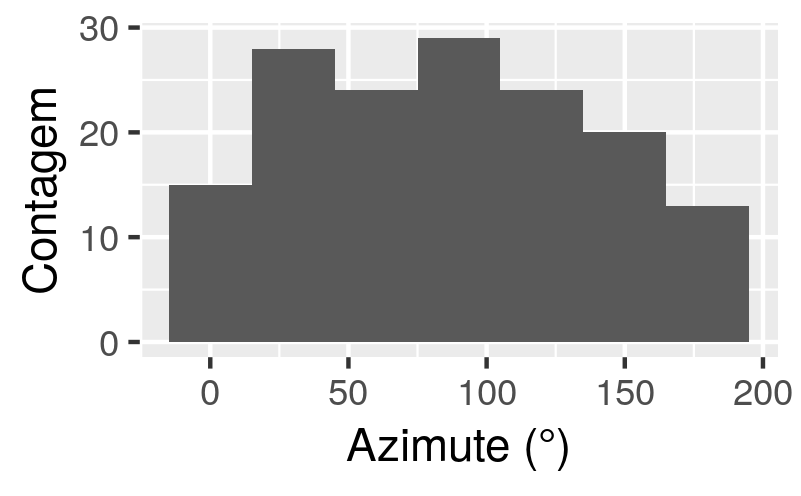
\includegraphics[width=\linewidth]{img/hist_azimute.png}
		\end{minipage}%
		\begin{minipage}{.5\textwidth}
			\centering
			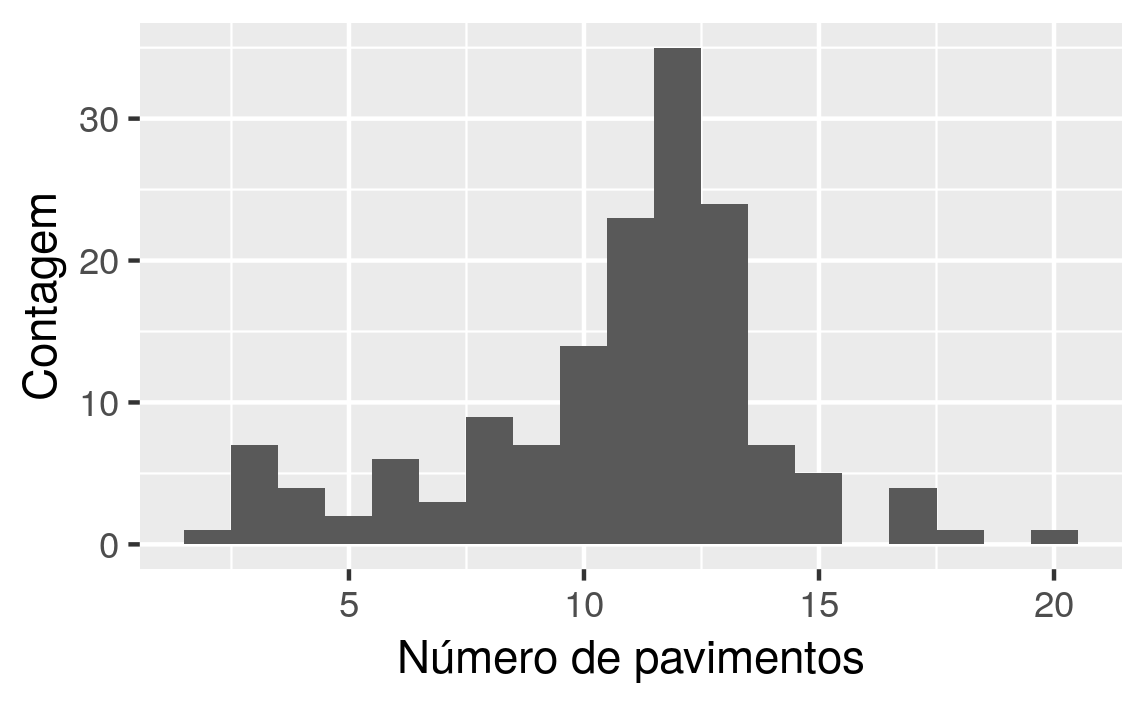
\includegraphics[width=\linewidth]{img/hist_numero_pavimentos.png}
		\end{minipage}
		\centering
		\begin{minipage}{.5\textwidth}
			\centering
			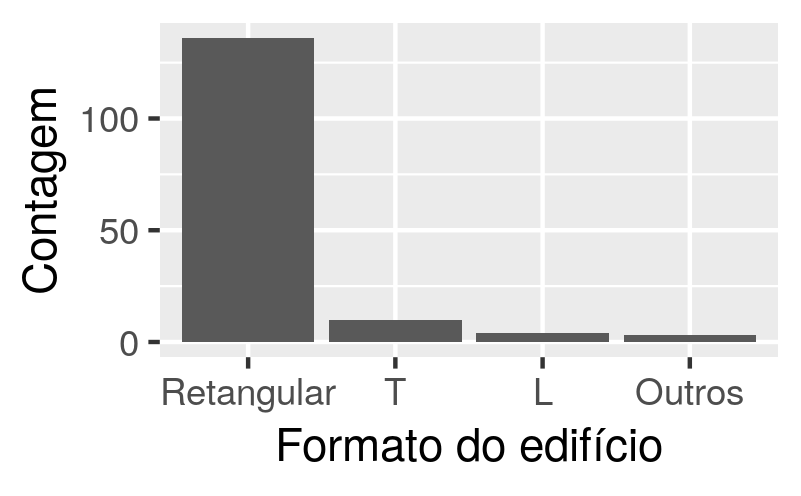
\includegraphics[width=\linewidth]{img/hist_formato.png}
		\end{minipage}%
		\begin{minipage}{.5\textwidth}
			\centering
			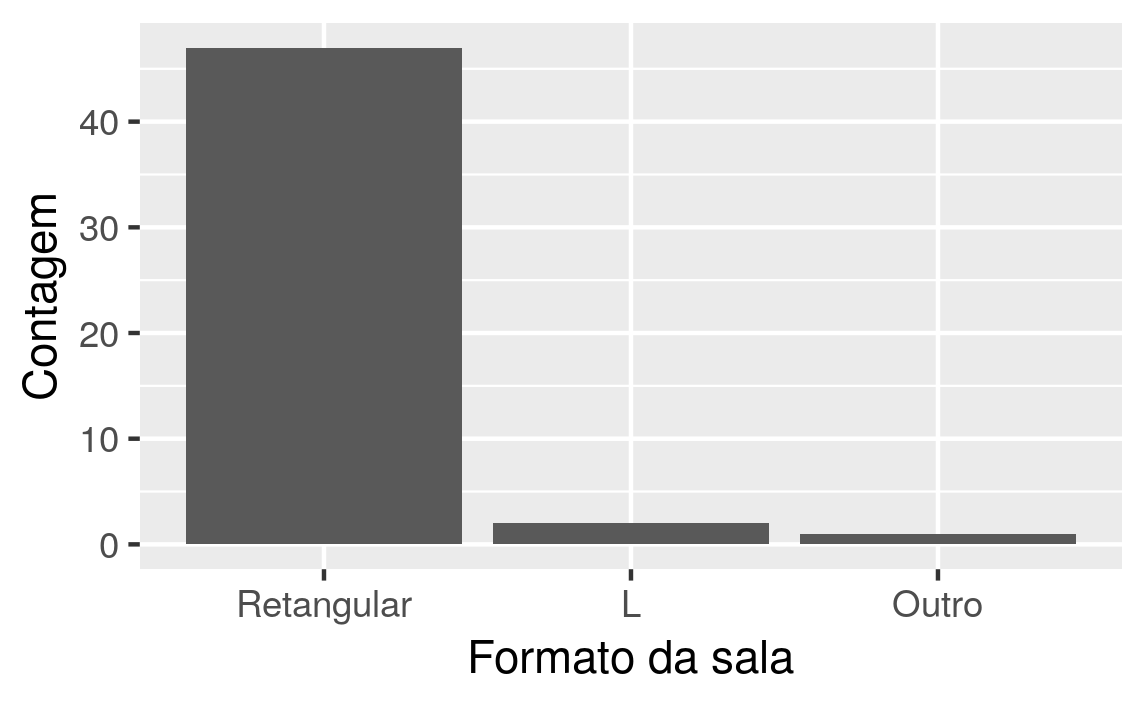
\includegraphics[width=\linewidth]{img/hist_formato_sala.png}
		\end{minipage}
		\centering
		\begin{minipage}{.5\textwidth}
			\centering
			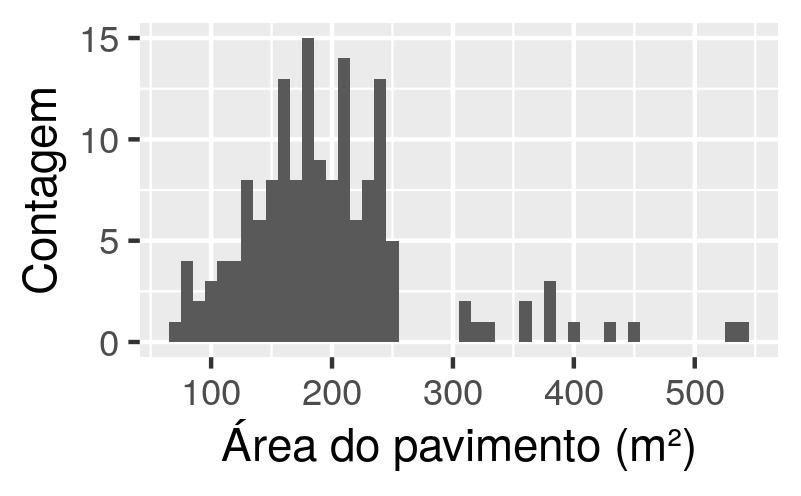
\includegraphics[width=\linewidth]{img/hist_area_edificio.png}
		\end{minipage}%
		\begin{minipage}{.5\textwidth}
			\centering
			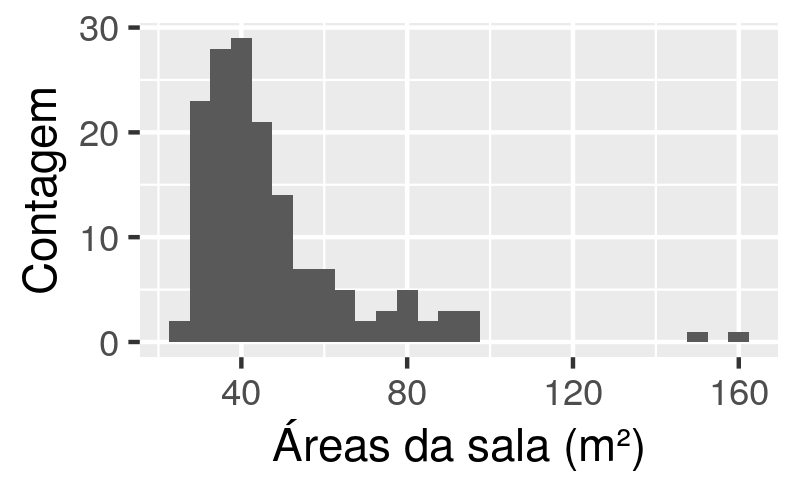
\includegraphics[width=\linewidth]{img/hist_area_zonas.png}
		\end{minipage}
		\centering
		\begin{minipage}{.5\textwidth}
			\centering
			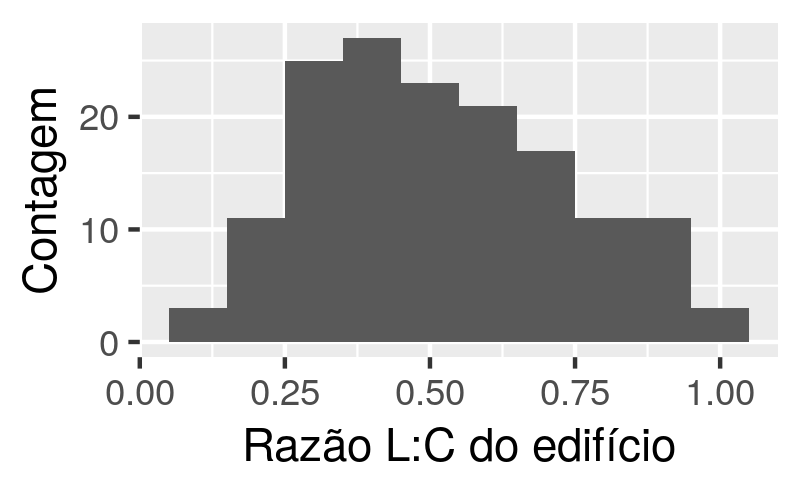
\includegraphics[width=\linewidth]{img/hist_ratio_edificio.png}
		\end{minipage}%
		\begin{minipage}{.5\textwidth}
			\centering
			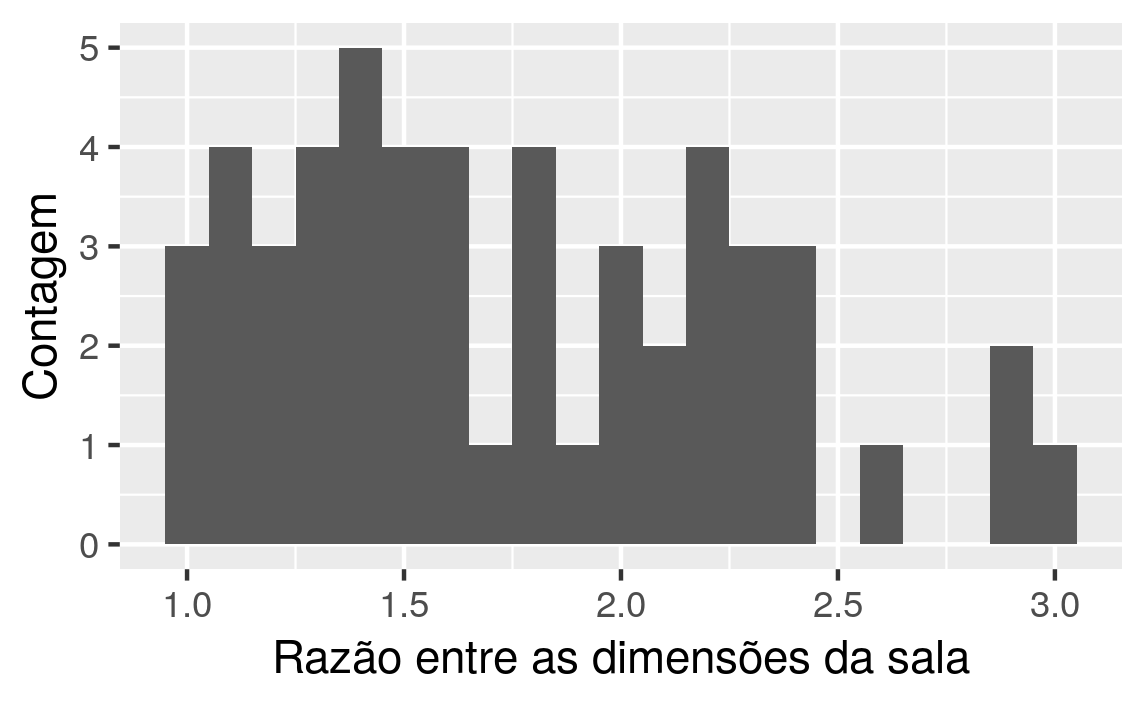
\includegraphics[width=\linewidth]{img/hist_ratio_sala.png}
		\end{minipage}
	\end{figure}
	\begin{figure}
		\captionof{figure}{Continuação}
		\label{fig:db_hist}
		\centering	
		\begin{minipage}{.5\textwidth}
			\centering
			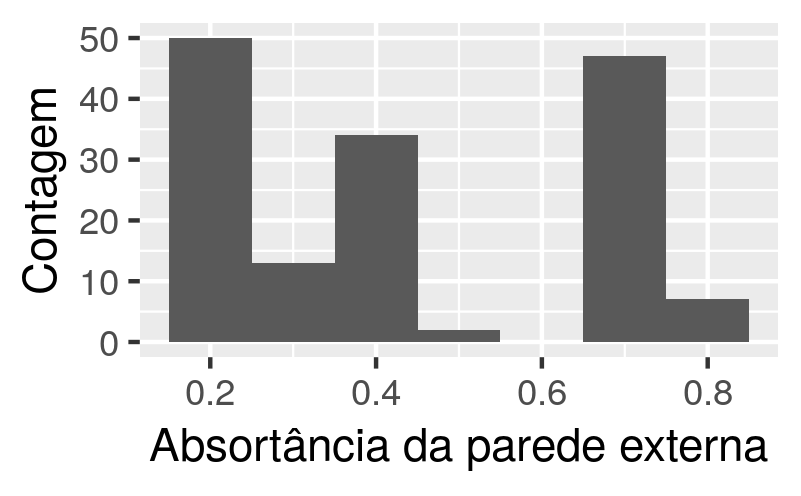
\includegraphics[width=\linewidth]{img/hist_absortancia.png}
		\end{minipage}%
		\begin{minipage}{.5\textwidth}
			\centering
			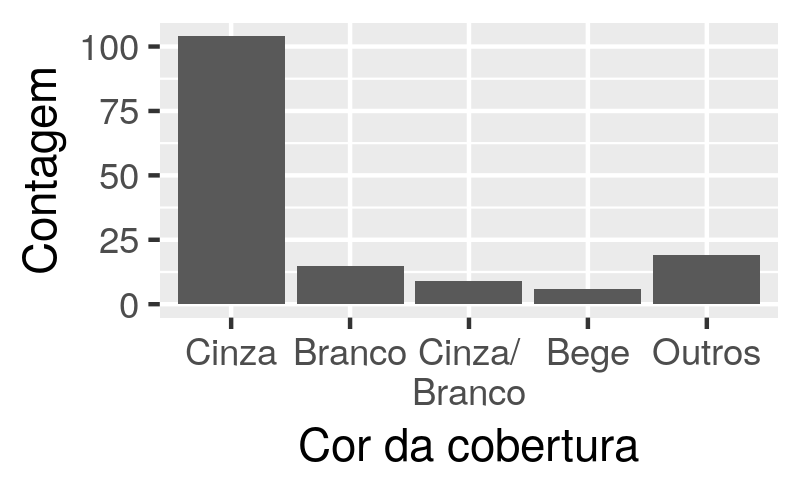
\includegraphics[width=\linewidth]{img/hist_cor_cobertura.png}
		\end{minipage}
		\centering	
		\begin{minipage}{.5\textwidth}
			\centering
			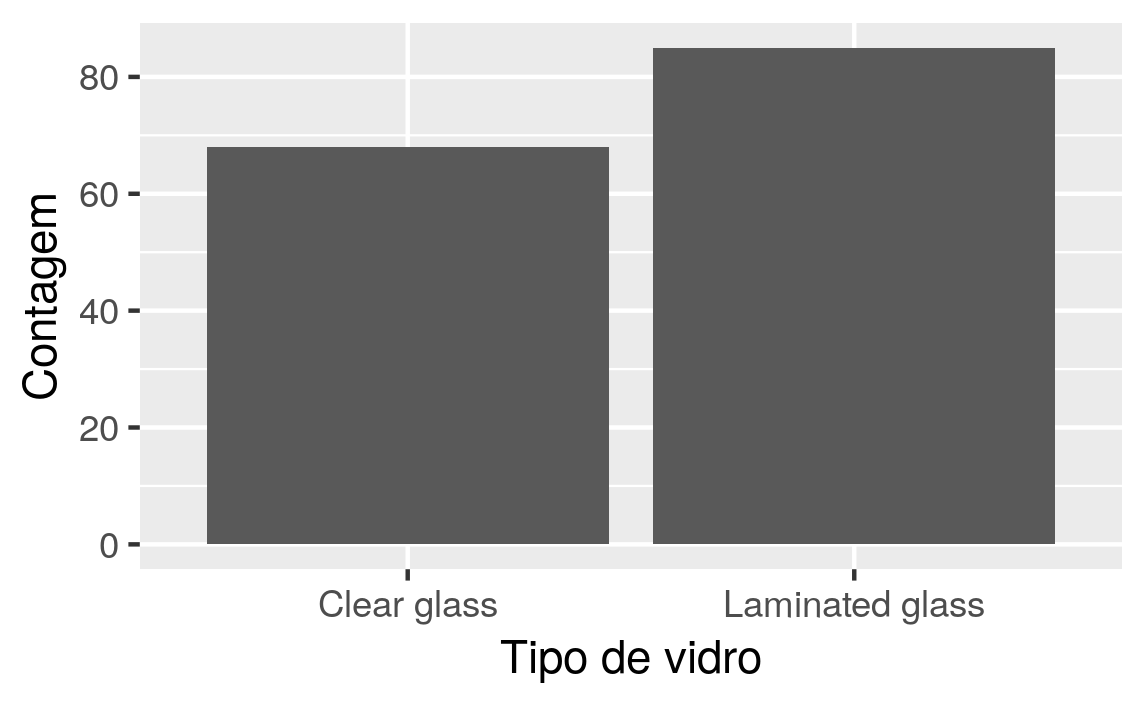
\includegraphics[width=\linewidth]{img/hist_tipo_vidro.png}
		\end{minipage}%
		\begin{minipage}{.5\textwidth}
			\centering
			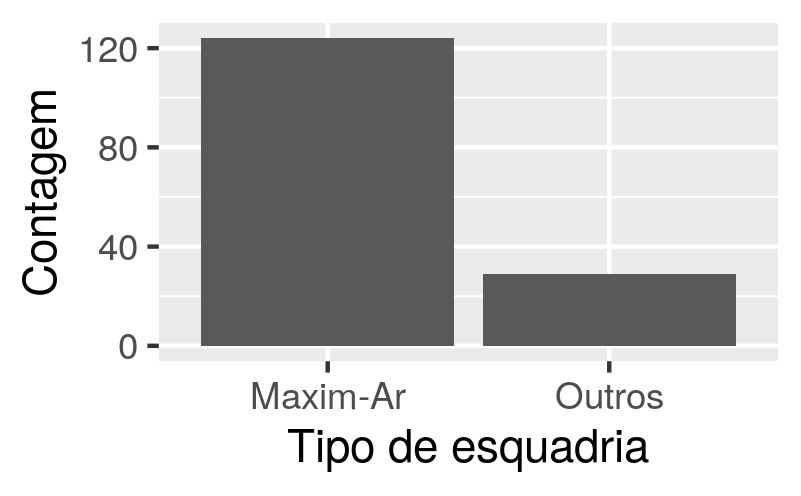
\includegraphics[width=\linewidth]{img/hist_esquadria.png}
		\end{minipage}
		\centering	
		\begin{minipage}{.5\textwidth}
			\centering
			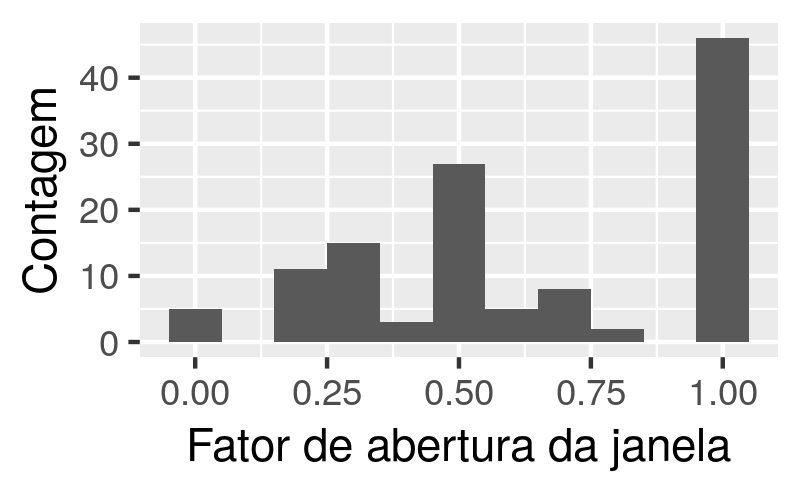
\includegraphics[width=\linewidth]{img/hist_openfac.png}
		\end{minipage}%
		\begin{minipage}{.5\textwidth}
			\centering
			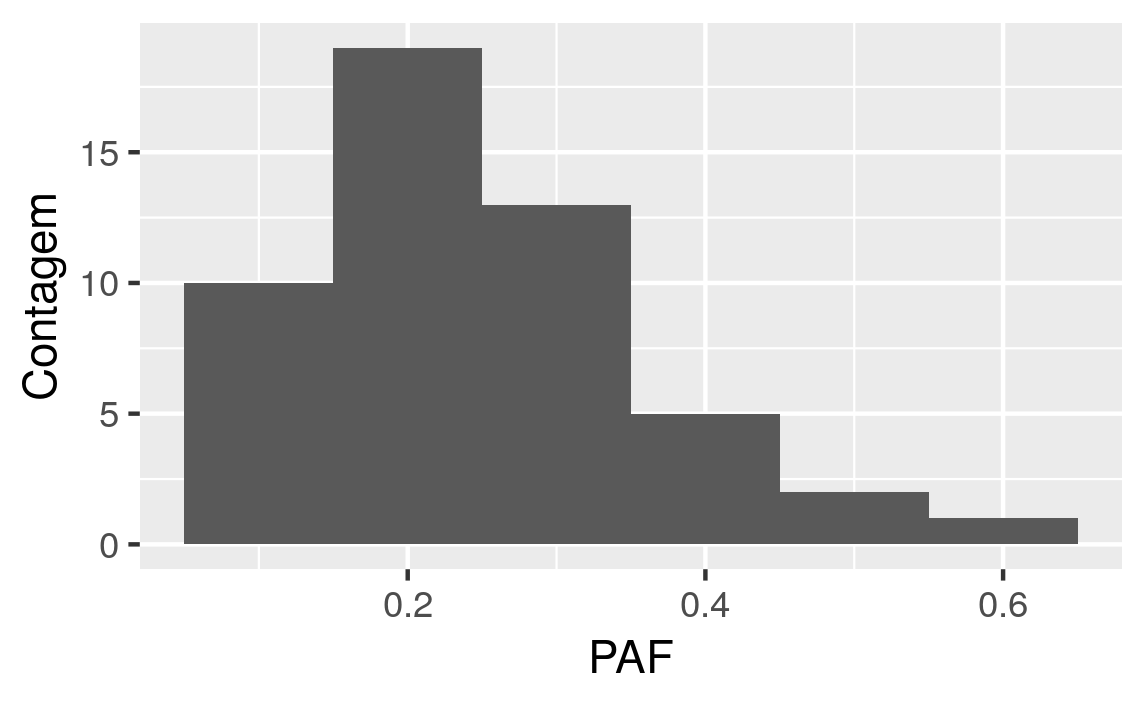
\includegraphics[width=\linewidth]{img/hist_PAF.png}
		\end{minipage}
		\centering	
		\begin{minipage}{.5\textwidth}
			\centering
			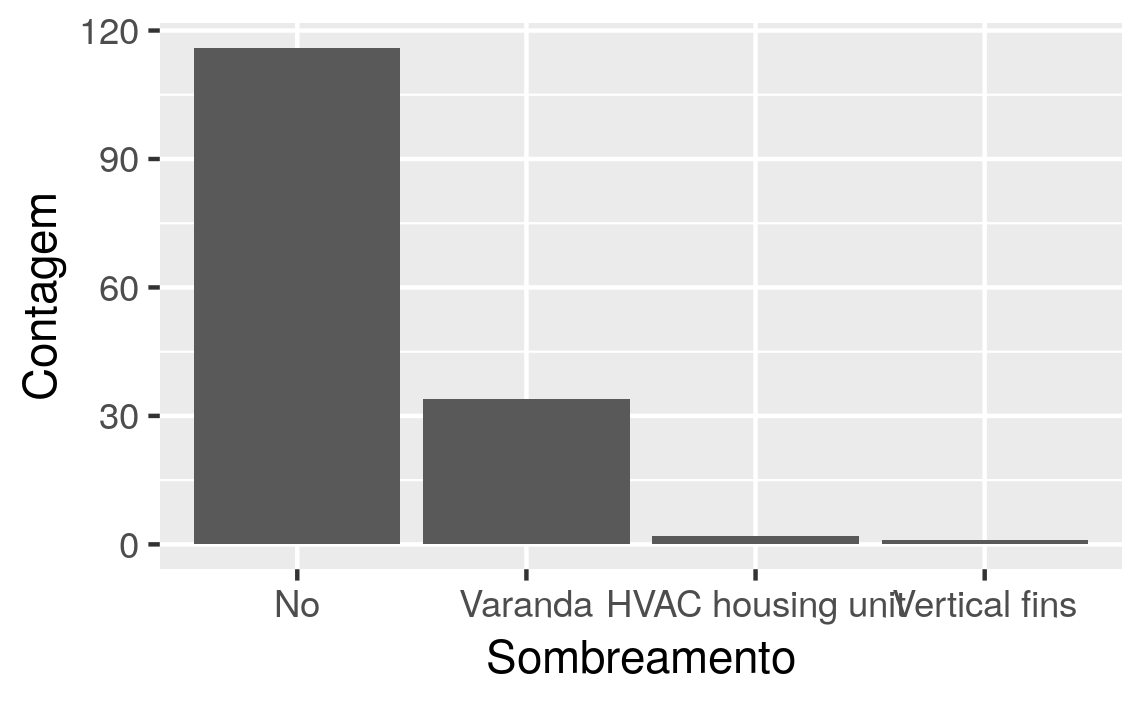
\includegraphics[width=\linewidth]{img/hist_sombreamento.png}
		\end{minipage}%
		\begin{minipage}{.5\textwidth}
			\centering
			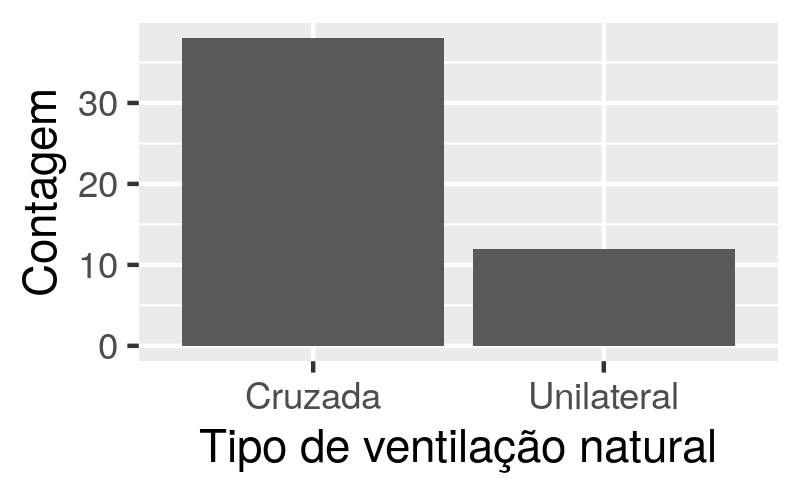
\includegraphics[width=\linewidth]{img/hist_tipo_vn.png}
		\end{minipage}
	\end{figure}
	
	Tanto os edifícios, quanto as salas existentes no banco de dados apresentam predominantemente formato retangular, a partir do qual considera-se que definir as simulações baseadas em modelos de edificações retangulares, como salas retangulares, representa adequadamente as tipologias de edifícios encontradas na cidade de São Paulo.
	
	A absortância da cobertura foi definida com o valor fixo de 0,7, valor aproximado para uma cobertura de cor cinza.
	
	Observou-se que esquadrias do tipo maxim-ar são predominante. Os objetos do \textit{Airflow Network} não modelam especificamente este tipo de esquadria. Porém, optou-se por considerar as janelas como não pivotantes. Considerar uma janela como horizontalmente pivotante implicaria na consideração de que a abertura acontece simultaneamente em cima e embaixo da janela. No caso da janela maxim-ar, por mais que a abertura aconteça em um eixo horizontal, ela abre apenas por baixo.
	
	O uso de elementos de sombreamento é pouco explorado nas edificações existentes. De qualquer maneira, considerou-se a modelagem de sombreamento horizontal sobre as aberturas da edificação, por considerar o potencial do sombreamento para bloquear a entrada de radiação nas zonas térmicas simuladas. Esse parâmetro foi variado a partir do ângulo de sombreamento formado entre a base da abertura e a proteção solar, localizada no topo da abertura.
	
	As informações relacionadas ao tipo de vidro não permitem definir valores relacionados ao fator solar. Observa-se apenas a ocorrência de vidros laminados e vidro comum incolor. Optou-se por variar o fator solar dos vidros nas simulações para avaliar o impacto deste parâmetro nos resultados de conforto térmico.
	
	A maioria das salas observadas possuem ventilação cruzada, mas a ventilação unilateral é uma estratégia com ocorrência considerável.
	
	Os demais parâmetros observados variaram continuamente de acordo com as distribuições obtidas. Como modelou-se apenas um pavimento nas simulações de referência, o parâmetro relacionado ao número de pavimento das edificações foi transformado no parâmetro "altura do pavimento".
	
	A Tabela \ref{table:param_def} apresenta os limites mínimos e máximos atribuídos aos diferentes parâmetros contínuos variados nas simulações, assim como os parâmetros variados pela lógica "sim/não". A velocidade do ar foi variada com valores discretos, de acordo com a Tabela \ref{table:var} do Capítulo \ref{chapter:metodologia}.
	
		\begin{table}[h]
			\centering
			\caption{Parâmetros com valores constantes.}
			\label{table:param_def}
			\begin{tabular}{|l |r |}
				\hline
				\textbf{Parâmetro} & \textbf{Valores} \\
				\hline
				Área da sala (m$^2$) & 20 - 100 \\
				\hline
				Razão L:C da sala (-) & 0,4 - 2,5 \\
				\hline
				Pé-direito (m) & 2,3 - 3,2 \\
				\hline
				Azimute ($^{\circ}$) & 0 - 360 \\
				\hline
				Altura do pavimento (m) & 0 - 50 \\
				\hline 
				Absortância da parede (-) & 0,2 - 0,8 \\
				\hline 
				Transmitância da parede (W/m$^2$K) & 0,5 - 4,4 \\
				\hline 
				Capacidade térmica da parede (kJ/m$^2$K) & 0,22 - 450,00 \\
				\hline 
				PAF (-) & 0,1 - 0,6 \\
				\hline 
				Fator solar do vidro (-) & 0,20 - 0,87 \\
				\hline 
				Sombreamento ($^{\circ}$) & 0 - 80 \\
				\hline 
				Densidade de ocupação (pessoa/m$^2$) & 0,05 - 0,20 \\
				\hline 
				Fator de abertura da janela (-) & 0,2 - 1,0 \\
				\hline 
				Razão L:C do edifício (-) & 0,2 - 1,0 \\
				\hline 
				Cobertura exposta & Sim / Não\\
				\hline 
				Piso exposto & Sim / Não\\
				\hline 
				Ventilação & Cruzada / Unilateral\\
				\hline 
				Velocidade do ar (m/s) & 0,0 - 1,2 \\
				\hline 
			\end{tabular}
%			\begin{flushleft}
%				Fonte: \citeauthoronline{INIC} \cite{INIC}, adaptado pelo autor.
%			\end{flushleft}				
		\end{table}
		
		
		\begin{equation}
		\label{eq:EHF}
		EHF = \frac{timesteps_{sup}}{timesteps_{ocup}}
		\end{equation}
	
		
		\begin{figure}[h]
			\centering
			\caption{Croqui da tipologia base}
			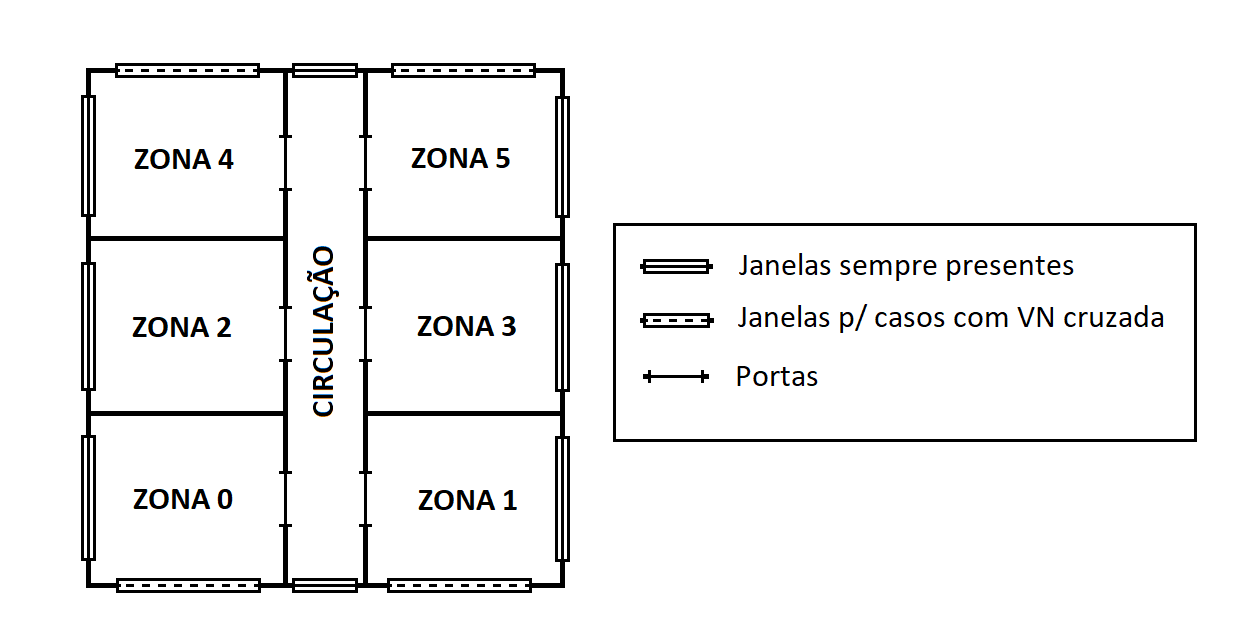
\includegraphics[width=1\linewidth]{img/croqui_07-11.png}
			\label{fig:croqui}
%			\begin{flushleft}
%				Fonte: o autor.
%			\end{flushleft}
		\end{figure}

\bibliography{citacoes}
	
\end{document}